% ============================================================================
% Chuong 3: PHAN TICH VA THIET KE HE THONG
% ============================================================================

\chapter{PHÂN TÍCH VÀ THIẾT KẾ HỆ THỐNG}
\label{ch:design}

Chương này đi từ mô hình mối đe dọa và các yêu cầu suy ra từ nó, qua kiến trúc
phần mềm và luồng dữ liệu, tới thiết kế cơ sở dữ liệu, quy trình phản hồi và thiết
kế giao diện vận hành. Mục tiêu là làm rõ \emph{tại sao} hệ thống được tổ chức như
vậy trước khi trình bày cách hiện thực ở Chương~\ref{ch:impl}.

\section{Mô hình mối đe dọa và yêu cầu hệ thống}
\label{sec:threat-model}

Thiết kế của hệ thống được dẫn dắt bởi một mô hình mối đe dọa cụ thể thay vì các
giả định chung chung. \emph{Tài sản} cần bảo vệ là các pod và dịch vụ trong namespace
mục tiêu của cụm. \emph{Kẻ tấn công} được giả định là một pod đã bị chiếm quyền điều
khiển bên trong cụm --- tình huống hoàn toàn thực tế khi một dịch vụ phơi ra Internet
bị khai thác --- và từ chỗ đứng đó kẻ tấn công tiến hành quét cổng theo chiều dọc
(nhiều cổng trên một đích) và theo chiều ngang (một cổng trên nhiều đích) nhằm lập
bản đồ mạng nội bộ, rồi dịch chuyển ngang tới các pod khác. \emph{Khả năng quan sát}
của hệ thống dựa trên một sự thật kiến trúc: mọi kết nối TCP của mọi pod đều phải đi
qua nhân Linux của nút chứa nó, do đó một bộ thu thập eBPF đặt ở tầng nhân quan sát
được trọn vẹn lưu lượng mà không cần thay đổi ứng dụng. Mô hình giả định CNI có hỗ
trợ \texttt{NetworkPolicy}, nhân có BTF, lưu lượng là IPv4, và kẻ tấn công chỉ có
quyền bên trong pod chứ không có quyền root trên nút; các tình huống nằm ngoài mô
hình --- tấn công ở tầng ứng dụng (L7), khai thác lỗ hổng nhân, hay kẻ tấn công đã
thoát khỏi container --- được ghi nhận tường minh là giới hạn phạm vi.

Từ mô hình trên, các tác nhân và chức năng của hệ thống được xác định. Người vận
hành an ninh (\textit{analyst}) tương tác với hệ thống để theo dõi cảnh báo, điều tra
sự cố và phê duyệt hành động phản hồi; hệ thống tự động đảm nhiệm việc thu thập, phát
hiện, tạo sự cố và sinh bản nháp chính sách. Hình~\ref{fig:usecase-soc} mô tả các
trường hợp sử dụng (\textit{use case}) chính theo các tác nhân, còn
Hình~\ref{fig:bfd} phân rã hệ thống thành các nhóm chức năng. Từ đó, các \emph{yêu cầu
chức năng} cốt lõi gồm: thu thập sự kiện kết nối ở tầng nhân; phát hiện quét cổng và
dịch chuyển ngang theo thời gian thực; tạo và làm giàu sự cố; sinh chính sách cách ly
theo cơ chế có người duyệt; và cung cấp giao diện theo dõi/xử lý. Các \emph{yêu cầu
phi chức năng} quan trọng gồm: chi phí thu thập đủ thấp để chạy thường trực trên mọi
nút, độ trễ phát hiện$\rightarrow$phản hồi ở mức giây, và khả năng tái lập trên cụm
thật --- những tiêu chí này được kiểm chứng định lượng ở Chương~\ref{ch:eval}.

\begin{figure}[H]
  \centering
  \resizebox{0.9\linewidth}{!}{% Sơ đồ use-case hệ thống SOC. Dùng ở Chương 3.
\begin{tikzpicture}[
    every node/.style={font=\small},
    uc/.style={draw, ellipse, fill=blue!8, align=center, minimum width=3.4cm,
               minimum height=1.0cm, inner sep=2pt, font=\footnotesize},
    act/.style={align=center, font=\footnotesize},
    rel/.style={-, shorten >=1pt, shorten <=1pt},
  ]
  % --- Actor: stick figure macro (vẽ tay) ---
  \newcommand{\actor}[3]{% (#1=name id)(#2=x,y)(#3=label)
    \begin{scope}[shift={#2}]
      \draw[thick] (0,0.55) circle (0.16);
      \draw[thick] (0,0.39) -- (0,-0.15);
      \draw[thick] (-0.22,0.18) -- (0.22,0.18);
      \draw[thick] (0,-0.15) -- (-0.18,-0.5);
      \draw[thick] (0,-0.15) -- (0.18,-0.5);
      \node[act] (#1) at (0,-0.95) {#3};
    \end{scope}}

  \actor{analyst}{(0,4.6)}{Chuyên viên\\phân tích (Analyst)}
  \actor{admin}{(0,0.6)}{Quản trị viên\\(Admin)}
  \actor{attacker}{(12.4,2.6)}{Kẻ tấn công\\(external)}

  % --- 6 use-case, gian cach doc 1.55cm de khong chong nhau ---
  \node[uc] (u1) at (6.4,6.3) {Xem dashboard\\\& cảnh báo};
  \node[uc] (u2) at (6.4,4.75) {Xem chi tiết\\sự cố};
  \node[uc] (u3) at (6.4,3.2) {Xác nhận / đóng\\sự cố};
  \node[uc] (u4) at (6.4,1.65) {Duyệt hành động\\phản hồi};
  \node[uc] (u5) at (6.4,0.1) {Cách ly Pod\\(NetworkPolicy)};
  \node[uc] (u6) at (6.4,-1.45) {Cấu hình ngưỡng\\\& người dùng};

  % --- System boundary ---
  \node[draw, rounded corners, fit={(4.5,-2.4) (8.3,7.4)}, inner sep=0pt,
        label={[font=\small\bfseries]above:Hệ thống SOC K8sSecDaP}] (sys) {};

  % analyst relations
  \foreach \u in {u1,u2,u3} \draw[rel] (analyst) -- (\u);
  % admin relations
  \foreach \u in {u2,u4,u5,u6} \draw[rel] (admin) -- (\u);

  % attacker triggers detection indirectly (dashed) -> noi toi bien he thong, tranh cat UC
  \draw[rel, dashed] (attacker) -- node[below, font=\scriptsize, pos=0.55]{sinh lưu lượng quét} (u1.east);
\end{tikzpicture}
}
  \caption{Sơ đồ use-case của hệ thống.}
  \label{fig:usecase-soc}
\end{figure}

\begin{figure}[H]
  \centering
  \resizebox{0.92\linewidth}{!}{% Sơ đồ phân rã chức năng (BFD) của nền tảng SOC K8sSecDaP. Dùng ở Chương 3.
\begin{tikzpicture}[
    every node/.style={font=\small},
    root/.style={draw, rounded corners=2pt, fill=blue!12, align=center,
                 minimum width=4.6cm, minimum height=0.9cm},
    grp/.style={draw, rounded corners=2pt, fill=green!12, align=center,
                minimum width=2.6cm, minimum height=0.85cm},
    leaf/.style={draw, align=center, fill=gray!6, font=\footnotesize,
                 minimum width=2.6cm, minimum height=0.72cm},
    edge/.style={-, thick},
  ]
  \node[root] (r) {Nền tảng giám sát \& phản hồi\\an ninh K8sSecDaP};

  \node[grp, below=1.0cm of r, xshift=-6.2cm] (g1) {1. Thu thập\\sự kiện};
  \node[grp, right=0.55cm of g1] (g2) {2. Phát hiện\\bất thường};
  \node[grp, right=0.55cm of g2] (g3) {3. Quản lý\\sự cố};
  \node[grp, right=0.55cm of g3] (g4) {4. Phản hồi\\chính sách};
  \node[grp, right=0.55cm of g4] (g5) {5. Quan sát\\\& kiểm toán};

  \draw[edge] (r) -- (g1); \draw[edge] (r) -- (g2); \draw[edge] (r) -- (g3);
  \draw[edge] (r) -- (g4); \draw[edge] (r) -- (g5);

  % --- Cot 1 ---
  \node[leaf, below=0.7cm of g1] (l1) {1.1 eBPF kprobe\\\texttt{tcp\_v4\_connect}};
  \node[leaf, below=0.25cm of l1] (l1b) {1.2 Chuẩn hoá\\sự kiện};
  % --- Cot 2 (3 chuc nang con) ---
  \node[leaf, below=0.7cm of g2] (l2) {2.1 Đếm tần suất\\(CMS) port-scan};
  \node[leaf, below=0.25cm of l2] (l2b) {2.2 Đồ thị\\SCC / blast-radius};
  \node[leaf, below=0.25cm of l2b] (l2c) {2.3 Ngưỡng \&\\cửa sổ thời gian};
  % --- Cot 3 ---
  \node[leaf, below=0.7cm of g3] (l3) {3.1 Vòng đời\\sự cố};
  \node[leaf, below=0.25cm of l3] (l3b) {3.2 Làm giàu\\IP$\rightarrow$Pod};
  % --- Cot 4 (3 chuc nang con) ---
  \node[leaf, below=0.7cm of g4] (l4) {4.1 Sinh\\NetworkPolicy};
  \node[leaf, below=0.25cm of l4] (l4b) {4.2 Duyệt \&\\áp cách ly};
  \node[leaf, below=0.25cm of l4b] (l4c) {4.3 Kiểm chứng\\cách ly};
  % --- Cot 5 ---
  \node[leaf, below=0.7cm of g5] (l5) {5.1 Dashboard\\Grafana};
  \node[leaf, below=0.25cm of l5] (l5b) {5.2 Nhật ký\\kiểm toán};

  % Noi tung chuc nang cha -> chuoi chuc nang con (1 -> 1.1 -> 1.2 ...)
  \draw[edge] (g1) -- (l1);  \draw[edge] (l1) -- (l1b);
  \draw[edge] (g2) -- (l2);  \draw[edge] (l2) -- (l2b); \draw[edge] (l2b) -- (l2c);
  \draw[edge] (g3) -- (l3);  \draw[edge] (l3) -- (l3b);
  \draw[edge] (g4) -- (l4);  \draw[edge] (l4) -- (l4b); \draw[edge] (l4b) -- (l4c);
  \draw[edge] (g5) -- (l5);  \draw[edge] (l5) -- (l5b);
\end{tikzpicture}
}
  \caption{Sơ đồ phân rã chức năng (BFD) của nền tảng giám sát an ninh.}
  \label{fig:bfd}
\end{figure}

Bảng~\ref{tab:bfd-leaf} đặc tả từng chức năng lá của sơ đồ phân rã --- nêu rõ nhiệm vụ cụ
thể của mỗi nút lá, làm cầu nối giữa phân rã chức năng và thiết kế thành phần ở các mục sau.

\begin{table}[H]
  \centering
  \caption{Đặc tả các chức năng lá của sơ đồ phân rã chức năng (BFD).}
  \label{tab:bfd-leaf}
  \small
  \begin{tabularx}{\linewidth}{@{}l l X@{}}
    \toprule
    \textbf{Mã} & \textbf{Chức năng lá} & \textbf{Nhiệm vụ} \\
    \midrule
    1.1 & eBPF kprobe \texttt{tcp\_v4\_connect} & Bắt mọi lời gọi \texttt{connect()} TCP/IPv4 ở tầng nhân trên mỗi nút \\
    1.2 & Chuẩn hoá sự kiện           & Trích src/dst/cổng/pid/thời gian, lọc theo nhãn vùng mạng, xuất JSON \\
    2.1 & Đếm tần suất (CMS)          & Cập nhật Count-Min Sketch theo địa chỉ nguồn, ước lượng số kết nối \\
    2.2 & Đồ thị SCC / blast-radius   & Dựng đồ thị giao tiếp, chạy Tarjan và BFS để tìm chu trình và bán kính \\
    2.3 & Ngưỡng \& cửa sổ thời gian  & So sánh tần suất với ngưỡng trên cửa sổ trượt, quyết định phát cảnh báo \\
    3.1 & Vòng đời sự cố              & Tạo, gộp trùng, cập nhật trạng thái (new/ack/resolved) của sự cố \\
    3.2 & Làm giàu IP$\rightarrow$Pod & Ánh xạ địa chỉ nguồn về tên pod và namespace qua API Kubernetes \\
    4.1 & Sinh NetworkPolicy         & Tạo bản nháp chính sách egress-deny gắn nhãn lên pod tấn công \\
    4.2 & Duyệt \& áp cách ly         & Trình bản nháp cho người duyệt; khi đồng ý thì áp qua API Kubernetes \\
    4.3 & Kiểm chứng cách ly         & Xác minh pod tấn công mất kết nối đi ra sau khi áp chính sách \\
    5.1 & Dashboard Grafana          & Trực quan hóa số liệu và cảnh báo theo thời gian thực cho người vận hành \\
    5.2 & Nhật ký kiểm toán          & Ghi lại mọi thao tác trên sự cố/hành động phục vụ điều tra và tuân thủ \\
    \bottomrule
  \end{tabularx}
\end{table}

\subsection{Đặc tả use-case}
\label{subsec:uc-spec}

Bảng~\ref{tab:uc-list} liệt kê các use-case của hệ thống cùng tác nhân tương ứng. Tác
nhân \emph{Chuyên viên phân tích} (Analyst) và \emph{Quản trị viên} (Admin) là người dùng;
\emph{Hệ thống} đại diện cho các chức năng tự động (thu thập, phát hiện, sinh sự cố) chạy
không cần can thiệp. Sau bảng tổng hợp là đặc tả chi tiết của các use-case quan trọng nhất.

\begin{table}[H]
  \centering
  \caption{Danh sách use-case và tác nhân.}
  \label{tab:uc-list}
  \small
  \begin{tabularx}{\linewidth}{@{}l X l@{}}
    \toprule
    \textbf{Mã} & \textbf{Use-case} & \textbf{Tác nhân} \\
    \midrule
    UC-01 & Xem dashboard và cảnh báo            & Analyst, Admin \\
    UC-02 & Điều tra chi tiết sự cố              & Analyst, Admin \\
    UC-03 & Ghi nhận / đóng sự cố                & Analyst, Admin \\
    UC-04 & Duyệt và áp hành động phản hồi       & Admin \\
    UC-05 & Cấu hình ngưỡng phát hiện và người dùng & Admin \\
    UC-06 & Tra cứu nhật ký kiểm toán            & Analyst, Admin \\
    UC-S1 & Thu thập, phát hiện và sinh sự cố (tự động) & Hệ thống \\
    \bottomrule
  \end{tabularx}
\end{table}

\begin{table}[H]
  \centering
  \caption{Đặc tả use-case UC-02 --- Điều tra chi tiết sự cố.}
  \label{tab:uc02}
  \small
  \begin{tabularx}{\linewidth}{@{}>{\bfseries}l X@{}}
    \toprule
    Mã / Tên & UC-02 --- Điều tra chi tiết sự cố \\
    \midrule
    Tác nhân & Chuyên viên phân tích (Analyst) \\
    Mô tả & Người vận hành mở một sự cố để xem ngữ cảnh đã làm giàu, các cảnh báo liên quan và bán kính ảnh hưởng nhằm đánh giá mức độ nghiêm trọng. \\
    Tiền điều kiện & Đã đăng nhập; tồn tại ít nhất một sự cố trong hệ thống. \\
    Luồng chính &
      \begin{enumerate}[nosep,leftmargin=*]
        \item Analyst chọn một sự cố từ danh sách.
        \item Hệ thống truy vấn cơ sở dữ liệu lấy chi tiết sự cố.
        \item Hệ thống hiển thị siêu dữ liệu (địa chỉ nguồn, pod, nút, mức độ, nhãn).
        \item Hệ thống hiển thị danh sách cảnh báo liên quan và đồ thị bán kính ảnh hưởng.
        \item Analyst xem và đánh giá ngữ cảnh sự cố.
      \end{enumerate} \\
    Luồng thay thế & 2a. Không tìm thấy sự cố: hệ thống báo lỗi và quay lại danh sách. \\
    Hậu điều kiện & Sự cố được hiển thị đầy đủ; sẵn sàng cho thao tác ghi nhận/đóng hoặc duyệt phản hồi. \\
    \bottomrule
  \end{tabularx}
\end{table}

\begin{table}[H]
  \centering
  \caption{Đặc tả use-case UC-04 --- Duyệt và áp hành động phản hồi.}
  \label{tab:uc04}
  \small
  \begin{tabularx}{\linewidth}{@{}>{\bfseries}l X@{}}
    \toprule
    Mã / Tên & UC-04 --- Duyệt và áp hành động phản hồi \\
    \midrule
    Tác nhân & Quản trị viên (Admin) \\
    Mô tả & Admin xem xét bản nháp \texttt{NetworkPolicy} cách ly do hệ thống sinh ra và quyết định phê duyệt hay từ chối; khi phê duyệt, chính sách được áp vào cụm. \\
    Tiền điều kiện & Đã đăng nhập với quyền Admin; sự cố có một bản nháp hành động ở trạng thái chờ duyệt. \\
    Luồng chính &
      \begin{enumerate}[nosep,leftmargin=*]
        \item Admin mở sự cố và chọn hành động phản hồi chờ duyệt.
        \item Hệ thống hiển thị xem trước nội dung \texttt{NetworkPolicy} sẽ áp.
        \item Admin nhập lý do và bấm Phê duyệt.
        \item Hệ thống áp chính sách qua API Kubernetes (Calico thực thi).
        \item Hệ thống xác minh hiệu lực và cập nhật trạng thái hành động.
        \item Hệ thống ghi toàn bộ thao tác vào nhật ký kiểm toán.
      \end{enumerate} \\
    Luồng thay thế &
      3a. Admin từ chối: hệ thống đánh dấu từ chối, ghi kiểm toán, không áp chính sách.\newline
      4a. Lỗi áp chính sách: hệ thống ghi lỗi, giữ trạng thái chờ và thông báo. \\
    Hậu điều kiện & Pod tấn công bị cách ly (nếu phê duyệt); mọi quyết định đều có dấu vết kiểm toán. \\
    \bottomrule
  \end{tabularx}
\end{table}

\begin{table}[H]
  \centering
  \caption{Đặc tả use-case UC-05 --- Cấu hình ngưỡng phát hiện và người dùng.}
  \label{tab:uc05}
  \small
  \begin{tabularx}{\linewidth}{@{}>{\bfseries}l X@{}}
    \toprule
    Mã / Tên & UC-05 --- Cấu hình ngưỡng phát hiện và người dùng \\
    \midrule
    Tác nhân & Quản trị viên (Admin) \\
    Mô tả & Admin điều chỉnh tham số phát hiện (ngưỡng, độ dài cửa sổ, kích thước sketch) và quản lý tài khoản/vai trò người dùng. \\
    Tiền điều kiện & Đã đăng nhập với quyền Admin. \\
    Luồng chính &
      \begin{enumerate}[nosep,leftmargin=*]
        \item Admin mở trang cấu hình.
        \item Admin sửa tham số phát hiện hoặc thông tin người dùng/vai trò.
        \item Hệ thống kiểm tra hợp lệ và lưu cấu hình.
        \item Hệ thống áp dụng cấu hình mới cho pipeline và ghi kiểm toán.
      \end{enumerate} \\
    Luồng thay thế & 3a. Dữ liệu không hợp lệ: hệ thống báo lỗi và yêu cầu nhập lại. \\
    Hậu điều kiện & Cấu hình mới có hiệu lực; thay đổi được lưu vết. \\
    \bottomrule
  \end{tabularx}
\end{table}

\begin{table}[H]
  \centering
  \caption{Đặc tả use-case UC-01 --- Xem dashboard và cảnh báo.}
  \label{tab:uc01}
  \small
  \begin{tabularx}{\linewidth}{@{}>{\bfseries}l X@{}}
    \toprule
    Mã / Tên & UC-01 --- Xem dashboard và cảnh báo \\
    \midrule
    Tác nhân & Chuyên viên phân tích (Analyst), Quản trị viên (Admin) \\
    Mô tả & Người vận hành theo dõi tình hình an ninh nội cụm qua bảng điều khiển Grafana và danh sách cảnh báo/sự cố mới nhất. \\
    Tiền điều kiện & Đã đăng nhập; hệ thống đang thu thập và phát hiện. \\
    Luồng chính &
      \begin{enumerate}[nosep,leftmargin=*]
        \item Người vận hành mở trang tổng quan.
        \item Hệ thống truy vấn số liệu (Prometheus) và danh sách sự cố mới.
        \item Hệ thống hiển thị các biểu đồ thời gian thực và bảng hành động chờ duyệt.
        \item Người vận hành nắm bắt tình hình và chọn mục cần điều tra.
      \end{enumerate} \\
    Luồng thay thế & 2a. Nguồn số liệu tạm gián đoạn: hiển thị cảnh báo thiếu dữ liệu. \\
    Hậu điều kiện & Bức tranh tổng quan được hiển thị; sẵn sàng cho điều tra chi tiết (UC-02). \\
    \bottomrule
  \end{tabularx}
\end{table}

\begin{table}[H]
  \centering
  \caption{Đặc tả use-case UC-03 --- Ghi nhận / đóng sự cố.}
  \label{tab:uc03}
  \small
  \begin{tabularx}{\linewidth}{@{}>{\bfseries}l X@{}}
    \toprule
    Mã / Tên & UC-03 --- Ghi nhận / đóng sự cố \\
    \midrule
    Tác nhân & Chuyên viên phân tích (Analyst) \\
    Mô tả & Sau khi điều tra, người vận hành ghi nhận (\textit{ack}) sự cố đang xử lý hoặc đóng (\textit{resolve}) sự cố đã giải quyết. \\
    Tiền điều kiện & Đã đăng nhập; sự cố tồn tại và đang ở trạng thái mở. \\
    Luồng chính &
      \begin{enumerate}[nosep,leftmargin=*]
        \item Người vận hành mở chi tiết sự cố.
        \item Người vận hành chọn ``Ack'' hoặc ``Resolve''.
        \item Hệ thống cập nhật trạng thái sự cố trong cơ sở dữ liệu.
        \item Hệ thống ghi thao tác vào nhật ký kiểm toán.
      \end{enumerate} \\
    Luồng thay thế & 3a. Sự cố đã đổi trạng thái bởi người khác: hệ thống thông báo và làm mới. \\
    Hậu điều kiện & Trạng thái sự cố được cập nhật; thao tác có dấu vết kiểm toán. \\
    \bottomrule
  \end{tabularx}
\end{table}

\section{Kiến trúc phần mềm và luồng dữ liệu}
\label{ch:architecture}

Hệ thống được tổ chức theo kiến trúc phân lớp, mỗi lớp một trách nhiệm rõ ràng và
giao tiếp với nhau qua các giao diện ổn định. Hình~\ref{fig:arch-c4} trình bày kiến
trúc ở mức container (theo mô hình C4): ở mỗi nút, một bộ thu thập eBPF chạy dưới dạng
\texttt{DaemonSet} bắt sự kiện kết nối và đẩy lên bộ máy pipeline qua bộ đệm vòng; bộ
máy pipeline áp các giải thuật phát hiện và phát cảnh báo lên trục thông điệp NATS;
phía trung tâm, bộ tổng hợp (\textit{aggregator}) tương quan và khử trùng lặp cảnh báo
trên phạm vi toàn cụm, dịch vụ sự cố tạo và làm giàu sự cố rồi lưu vào PostgreSQL, còn
bộ sinh phản hồi tạo bản nháp
\texttt{NetworkPolicy}; cuối cùng, người vận hành theo dõi qua Grafana và thao tác qua
console web. Cách phân tách này cho phép thay thế hoặc nâng cấp từng thành phần độc
lập, đồng thời cô lập phần chạy đặc quyền (bộ thu thập tầng nhân) khỏi phần logic
nghiệp vụ.

Luồng dữ liệu xuyên suốt hệ thống được mô tả ở hai mức. Hình~\ref{fig:dfd0} cho cái
nhìn ngữ cảnh: dữ liệu khởi nguồn từ lưu lượng kết nối trong nhân, chảy qua hệ thống
xử lý và kết thúc ở người vận hành dưới dạng cảnh báo, sự cố và hành động phản hồi.
Hình~\ref{fig:dfd1} phân rã chi tiết hơn các tiến trình bên trong và các kho dữ liệu
mà chúng đọc/ghi. Riêng tuyến đường ``trên mỗi nút $\rightarrow$ xử lý tập trung''
--- đặc trưng của mô hình \texttt{DaemonSet} --- được làm rõ ở
Hình~\ref{fig:agent-flow}: phần chạy phân tán trên từng nút chỉ đảm nhiệm thu thập và
phát hiện cục bộ, còn việc hợp nhất, lưu trữ và hiển thị được tập trung hóa.

\begin{figure}[H]
  \centering
  \resizebox{0.72\linewidth}{!}{% Sơ đồ kiến trúc phân lớp (C4 - mức Container). Dùng ở Chương 3.
\begin{tikzpicture}[
    every node/.style={font=\footnotesize},
    comp/.style={draw, rounded corners=2pt, align=center, minimum width=2.9cm,
                 minimum height=0.95cm},
    kern/.style={comp, fill=red!12},
    proc/.style={comp, fill=blue!10},
    data/.style={comp, fill=orange!16},
    ui/.style={comp, fill=green!14},
    bus/.style ={draw, rounded corners=2pt, fill=orange!16, align=center,
                 minimum width=12.6cm, minimum height=0.85cm},
    flow/.style={-{Stealth[length=2.2mm]}, thick},
    lbl/.style={font=\scriptsize, fill=white, inner sep=1.5pt},
  ]
  % Hang 1: mat phang du lieu tren moi node (gian cach rong de nhan mui ten khong tran)
  \node[kern] (kprobe)    at (0,0)   {eBPF kprobe\\\texttt{tcp\_v4\_connect}};
  \node[proc] (collector) at (4.6,0) {Collector\\(libbpf, C++)};
  \node[proc] (pipeline)  at (9.2,0) {Pipeline engine\\CMS/Tarjan/BFS};

  % Bus NATS (thanh ngang rong) o giua
  \node[bus] (nats) at (4.6,-2.0) {NATS JetStream --- bus sự kiện / cảnh báo};

  % Hang 3: hai dich vu tieu thu
  \node[proc] (agg)      at (0,-4.0)   {Aggregator\\(đồ thị toàn cục)};
  \node[proc] (incident) at (9.2,-4.0) {Incident service\\(Go)};

  % Hang 4: luu tru + giao dien
  \node[ui]   (grafana) at (0,-6.0)   {Grafana\\(dashboard)};
  \node[ui]   (console) at (4.6,-6.0) {Web console\\(duyệt phản hồi)};
  \node[data] (pg)      at (9.2,-6.0) {PostgreSQL\\(sự cố/kiểm toán)};
  \node[kern] (k8s)     at (4.6,-7.7) {Kubernetes API\\(NetworkPolicy)};

  % Luong hang 1 (nhan DAT TREN mui ten, du khoang trong)
  \draw[flow] (kprobe.east)    -- node[lbl, above]{ring buf} (collector.west);
  \draw[flow] (collector.east) -- node[lbl, above]{JSON}     (pipeline.west);
  % Pipeline xuat ban xuong bus
  \draw[flow] (pipeline.south) -- (pipeline.south|-nats.north);
  % Bus -> 2 dich vu tieu thu (mui ten huong XUONG = tieu thu)
  \draw[flow] (nats.south-|agg.north)      -- (agg.north);
  \draw[flow] (nats.south-|incident.north) -- (incident.north);
  % Dich vu -> luu tru / giao dien
  \draw[flow] (agg)      -- (grafana);
  \draw[flow] (incident) -- (pg);
  % incident -> web console: thoat ben TRAI incident, di ngang roi xuong (khong trung incident->pg)
  \draw[flow] (incident.west) -- (console.north|-incident.west) -- (console.north);
  % Web console ap NetworkPolicy
  \draw[flow] (console) -- node[lbl, right]{apply} (k8s);
\end{tikzpicture}
}
  \caption{Kiến trúc mức container (mô hình C4).}
  \label{fig:arch-c4}
\end{figure}

\begin{figure}[H]
  \centering
  \resizebox{0.85\linewidth}{!}{% DFD mức ngữ cảnh (level 0). Dùng ở Chương 3.
\begin{tikzpicture}[
    node distance=2.0cm,
    every node/.style={font=\small},
    ext/.style={draw, fill=gray!10, minimum width=2.7cm, minimum height=1.0cm, align=center},
    proc/.style={draw, circle, fill=blue!12, align=center, minimum size=2.7cm, font=\footnotesize},
    store/.style={draw, fill=orange!14, align=center, minimum width=2.8cm, minimum height=0.8cm},
    flow/.style={-{Stealth[length=2.2mm]}, thick, font=\scriptsize},
  ]
  \node[ext] (kernel) {Nhân Linux\\trên các node};
  \node[proc, right=3.6cm of kernel] (soc) {Hệ thống\\SOC\\K8sSecDaP};
  \node[ext, right=3.6cm of soc] (analyst) {Chuyên viên\\phân tích};
  \node[store, below=2.0cm of soc] (db) {Kho sự cố \& kiểm toán};
  \node[ext, above=1.7cm of soc] (k8s) {Kubernetes API\\(NetworkPolicy)};

  \draw[flow] (kernel) -- node[above]{sự kiện \texttt{connect()}} (soc);
  % Hai chieu soc <-> analyst: tach thanh 2 cung cong, nhan tren/duoi ro rang
  \draw[flow] (soc) to[bend left=22] node[above, pos=0.5]{cảnh báo / sự cố} (analyst);
  \draw[flow] (analyst) to[bend left=22] node[below, pos=0.5]{duyệt phản hồi} (soc);
  \draw[flow] (soc) -- node[right]{ghi / đọc} (db);
  \draw[flow] (soc) -- node[right]{áp cách ly} (k8s);
\end{tikzpicture}
}
  \caption{Sơ đồ luồng dữ liệu mức ngữ cảnh (DFD level 0).}
  \label{fig:dfd0}
\end{figure}

\begin{figure}[H]
  \centering
  \resizebox{0.95\linewidth}{!}{% DFD mức 1 (phân rã tiến trình SOC). Dùng ở Chương 3.
\begin{tikzpicture}[
    node distance=1.0cm and 2.7cm,
    every node/.style={font=\footnotesize},
    proc/.style={draw, circle, fill=blue!12, align=center, minimum size=1.8cm},
    ext/.style={draw, fill=gray!10, align=center, minimum width=2.2cm, minimum height=0.9cm},
    store/.style={draw, fill=orange!14, align=center, minimum width=2.4cm, minimum height=0.7cm},
    flow/.style={-{Stealth[length=2mm]}, thick, font=\scriptsize},
  ]
  \node[ext] (kernel) {Nhân Linux\\(node)};
  \node[proc, right=of kernel] (p1) {1.0\\Thu thập};
  \node[proc, right=of p1] (p2) {2.0\\Phát hiện};
  \node[proc, right=of p2] (p3) {3.0\\Quản lý\\sự cố};
  \node[ext, right=of p3] (analyst) {Analyst};
  \node[proc, below=2.0cm of p3] (p4) {4.0\\Phản hồi};
  \node[ext, left=of p4] (k8s) {K8s API};

  % Kho du lieu: dat duoi tien trinh sinh ra no de tranh cat ngang
  \node[store, below=0.9cm of p1] (d2) {D2: cảnh báo};
  \node[store, below=0.9cm of p2] (d1) {D1: sự cố};

  \draw[flow] (kernel) -- node[above]{\texttt{connect()}} (p1);
  \draw[flow] (p1) -- node[above, align=center]{sự kiện\\chuẩn hoá} (p2);
  \draw[flow] (p2) -- node[above]{cảnh báo} (p3);
  \draw[flow] (p2) -- (d2);
  \draw[flow] (p3) to[bend right=10] (d1);
  \draw[flow] (p3) -- node[above]{hiển thị} (analyst);
  \draw[flow] (analyst.south) to[bend left=20] node[right]{duyệt} (p4.east);
  \draw[flow] (p3) -- node[right]{yêu cầu cách ly} (p4);
  \draw[flow] (p4) -- node[above]{NetworkPolicy} (k8s);
  \node[store, below=0.9cm of p4] (d3) {D3: kiểm toán};
  \draw[flow] (p4) -- (d3);
\end{tikzpicture}
}
  \caption{Sơ đồ luồng dữ liệu mức 1.}
  \label{fig:dfd1}
\end{figure}

Tiến trình phát hiện (2.0) --- phần lõi thuật toán của hệ thống --- được phân rã thêm một
mức ở Hình~\ref{fig:dfd2}: sự kiện sau khi phân loại địa chỉ (2.1) vừa được đếm tần suất
bằng Count-Min Sketch (2.2) vừa được dùng để phân tích đồ thị bằng Tarjan/BFS (2.3); cả
hai nhánh đọc/ghi trạng thái sketch và đồ thị, rồi hội tụ ở bước sinh cảnh báo (2.4).

\begin{figure}[H]
  \centering
  \resizebox{0.95\linewidth}{!}{% DFD muc 2: phan ra tien trinh 2.0 (Phat hien) cua pipeline. Chuong 3.
\begin{tikzpicture}[
    node distance=1.2cm and 1.7cm,
    every node/.style={font=\footnotesize},
    proc/.style={draw, circle, fill=blue!12, align=center, minimum size=1.85cm},
    ext/.style={draw, fill=gray!10, align=center, minimum width=1.9cm, minimum height=0.95cm},
    store/.style={draw, fill=orange!14, align=center, minimum width=3.7cm, minimum height=0.72cm},
    flow/.style={-{Stealth[length=2mm]}, thick, font=\scriptsize},
  ]
  % Hang tren: luong chinh in -> 2.1 -> 2.2 -> 2.4 -> 3.0
  \node[ext] (in) {1.0\\Thu thập};
  \node[proc, right=of in] (p1) {2.1\\Phân loại\\(LPM)};
  \node[proc, right=of p1] (p2) {2.2\\Đếm tần suất\\(CMS)};
  \node[proc, right=of p2] (p4) {2.4\\Sinh\\cảnh báo};
  \node[ext, right=of p4] (out) {3.0\\Quản lý\\sự cố};
  % Nhanh do thi 2.3 nam duoi 2.2; kho du lieu D nam duoi 2.3 (cach ro rang)
  \node[proc, below=1.75cm of p2] (p3) {2.3\\Phân tích\\đồ thị\\(Tarjan/BFS)};
  \node[store, below=0.95cm of p3] (d) {D: trạng thái sketch \& đồ thị};

  \draw[flow] (in) -- node[above]{sự kiện} (p1);
  \draw[flow] (p1) -- node[above]{$+$ nhãn vùng} (p2);
  \draw[flow] (p2) -- node[above]{vượt ngưỡng} (p4);
  \draw[flow] (p4) -- node[above]{cảnh báo} (out);
  % 2.1 -> 2.3 (re xuong nhanh do thi)
  \draw[flow] (p1.south) |- (p3.west);
  % 2.3 -> 2.4 (chu trinh / ban kinh): re phai roi len, di duoi 2.2
  \draw[flow] (p3.east) -| node[pos=0.28,below]{chu trình / bán kính} (p4.south);
  % 2.2 va 2.3 ghi/doc trang thai vao kho D
  \draw[flow] (p3) -- (d);
  \draw[flow] (p2.west) -- ++(-0.55,0) |- (d.west);
\end{tikzpicture}
}
  \caption{Sơ đồ luồng dữ liệu mức 2 (tiến trình phát hiện).}
  \label{fig:dfd2}
\end{figure}

\begin{figure}[H]
  \centering
  \resizebox{0.95\linewidth}{!}{% Workflow agent thu thập (DaemonSet) trên node → xử lý tập trung. Dùng ở Chương 3.
\begin{tikzpicture}[
    node distance=0.65cm,
    every node/.style={font=\footnotesize},
    astep/.style={draw, rounded corners=2pt, fill=blue!10, align=center,
                 minimum width=3.2cm, minimum height=0.8cm},
    cstep/.style={astep, fill=green!12},
    flow/.style={-{Stealth[length=2.2mm]}, thick},
  ]
  % Lane 1: trên mỗi node (DaemonSet)
  \node[astep] (s1) {connect() được gọi\\trong Pod};
  \node[astep, below=of s1] (s2) {kprobe bắt sự kiện,\\lọc src pod-network};
  \node[astep, below=of s2] (s3) {Đẩy qua ring buffer\\$\rightarrow$ collector};
  \node[astep, below=of s3] (s4) {Pipeline: CMS đếm,\\dựng đồ thị, sinh cảnh báo};

  % Lane 2: tập trung
  \node[cstep, right=3.6cm of s2] (c1) {NATS JetStream\\(bus tập trung)};
  \node[cstep, below=of c1] (c2) {Aggregator hợp nhất\\đồ thị đa node};
  \node[cstep, below=of c2] (c3) {Incident service\\tạo / làm giàu sự cố};
  \node[cstep, below=of c3] (c4) {Lưu PostgreSQL +\\hiển thị cho Analyst};

  \draw[flow] (s1) -- (s2);
  \draw[flow] (s2) -- (s3);
  \draw[flow] (s3) -- (s4);
  \draw[flow] (s4.east) -- node[above, font=\scriptsize]{publish alert} (c1.west|-s4);
  \draw[flow] (c1) -- (c2);
  \draw[flow] (c2) -- (c3);
  \draw[flow] (c3) -- (c4);

  % swimlane labels
  \node[font=\small\bfseries, above=0.2cm of s1] {Trên mỗi node — DaemonSet};
  \node[font=\small\bfseries, above=0.2cm of c1] {Xử lý tập trung};
\end{tikzpicture}
}
  \caption{Luồng xử lý phân tán trên mỗi nút (DaemonSet) và phần xử lý tập trung.}
  \label{fig:agent-flow}
\end{figure}

Một quyết định thiết kế quan trọng ở tầng pipeline là áp dụng mẫu thiết kế Strategy
kết hợp Registry \cite{gamma1995patterns}: mỗi họ giải thuật (ước lượng tần suất, phát
hiện thành phần liên thông mạnh, tính khả-đạt, phân loại địa chỉ) được trừu tượng hóa
thành một giao diện chung và đăng ký vào một sổ đăng ký; việc lựa chọn cài đặt cụ thể
được điều khiển hoàn toàn bằng tệp cấu hình YAML. Nhờ đó, có thể thay Count-Min Sketch
bằng một biến thể khác, hoặc đổi tham số cửa sổ và ngưỡng, mà không phải sửa và biên
dịch lại mã nguồn --- một đặc tính có giá trị cho cả việc thử nghiệm lẫn vận hành.

\subsection{Luồng gọi giữa các dịch vụ}
\label{subsec:sequences}

Để làm rõ trình tự tương tác giữa các thành phần, ba sơ đồ tuần tự (\textit{sequence
diagram}) dưới đây mô tả ba kịch bản chính. Hình~\ref{fig:seq-ingestion} là luồng
\emph{thu thập}: một lời gọi \texttt{connect()} trong pod bị kprobe bắt, bộ thu thập lọc
theo nhãn vùng mạng rồi đẩy sự kiện sang pipeline; pipeline cập nhật Count-Min Sketch và
phát cảnh báo khi vượt ngưỡng.

\begin{figure}[H]
  \centering
  \resizebox{0.86\linewidth}{!}{% Sequence: thu thap su kien (ingestion). Chuong 3.
\begin{tikzpicture}[font=\footnotesize, >={Stealth[length=2mm]},
    ll/.style ={draw, rounded corners=2pt, fill=blue!8, align=center,
                minimum height=0.95cm, minimum width=2.2cm},
    msg/.style={-{Stealth[length=2mm]}, thick},
  ]
  \def\yb{-5.6}
  \node[ll] (a) at (0,0)   {Pod\\(ứng dụng)};
  \node[ll] (b) at (3.6,0) {collector-eBPF\\(DaemonSet)};
  \node[ll] (c) at (7.2,0) {pipeline};
  \node[ll] (d) at (10.2,0){NATS};
  \foreach \n in {a,b,c,d}{ \draw[dashed, gray!60] (\n.south) -- ++(0,\yb); }

  \draw[msg] (0,-1.3)  -- node[above]{\texttt{connect()} --- kprobe bắt} (3.6,-1.3);
  % self: loc LPM
  \draw[msg] (3.6,-2.1) -- ++(0.7,0) -- ++(0,-0.45) -- (3.6,-2.55);
  \node[right, font=\scriptsize] at (4.3,-2.3) {lọc LPM (\texttt{src\_label}=1)};
  \draw[msg] (3.6,-3.15) -- node[above]{sự kiện JSON (ring buffer)} (7.2,-3.15);
  % self: CMS record + kiem nguong
  \draw[msg] (7.2,-3.95) -- ++(0.7,0) -- ++(0,-0.45) -- (7.2,-4.4);
  \node[right, font=\scriptsize] at (7.9,-4.15) {CMS \texttt{record}, kiểm ngưỡng};
  \draw[msg] (7.2,-5.0) -- node[above]{cảnh báo \texttt{port\_scan} (nếu vượt ngưỡng)} (10.2,-5.0);
\end{tikzpicture}
}
  \caption{Sơ đồ tuần tự: thu thập sự kiện và phát hiện quét cổng.}
  \label{fig:seq-ingestion}
\end{figure}

Hình~\ref{fig:seq-incident} là luồng \emph{tạo và làm giàu sự cố}: dịch vụ sự cố nhận
cảnh báo từ NATS, tạo sự cố, tra cứu API Kubernetes để ánh xạ địa chỉ nguồn về đúng pod,
lưu sự cố kèm ngữ cảnh vào PostgreSQL và sinh bản nháp chính sách cách ly.

\begin{figure}[H]
  \centering
  \resizebox{0.86\linewidth}{!}{% Sequence: tao + lam giau su co. Chuong 3.
\begin{tikzpicture}[font=\footnotesize, >={Stealth[length=2mm]},
    ll/.style ={draw, rounded corners=2pt, fill=blue!8, align=center,
                minimum height=0.72cm, minimum width=2.2cm},
    msg/.style={-{Stealth[length=2mm]}, thick},
    ret/.style={-{Stealth[length=2mm]}, thick, dashed},
  ]
  \def\yb{-6.0}
  \node[ll] (a) at (0,0)    {NATS};
  \node[ll] (b) at (3.4,0)  {incident-service};
  \node[ll] (c) at (7.4,0)  {K8s API};
  \node[ll] (d) at (10.6,0) {PostgreSQL};
  \foreach \n in {a,b,c,d}{ \draw[dashed, gray!60] (\n.south) -- ++(0,\yb); }

  \draw[msg] (0,-1.3) -- node[above]{cảnh báo \texttt{port\_scan}} (3.4,-1.3);
  % self: tao su co
  \draw[msg] (3.4,-2.1) -- ++(0.7,0) -- ++(0,-0.45) -- (3.4,-2.55);
  \node[right, font=\scriptsize] at (4.1,-2.3) {tạo sự cố};
  \draw[msg] (3.4,-3.15) -- node[above]{tra cứu pod theo \texttt{src\_ip}} (7.4,-3.15);
  \draw[ret] (7.4,-3.75) -- node[above]{pod (tên, namespace)} (3.4,-3.75);
  \draw[msg] (3.4,-4.45) -- node[above]{lưu sự cố $+$ ngữ cảnh pod} (10.6,-4.45);
  % self: sinh ban nhap NetworkPolicy
  \draw[msg] (3.4,-5.25) -- ++(0.7,0) -- ++(0,-0.45) -- (3.4,-5.7);
  \node[right, font=\scriptsize] at (4.1,-5.45) {sinh bản nháp \texttt{NetworkPolicy}};
\end{tikzpicture}
}
  \caption{Sơ đồ tuần tự: tạo và làm giàu sự cố.}
  \label{fig:seq-incident}
\end{figure}

Hình~\ref{fig:seq-response} là luồng \emph{phê duyệt và áp phản hồi}: quản trị viên phê
duyệt qua console, dịch vụ sự cố áp \texttt{NetworkPolicy} qua API Kubernetes, cập nhật
trạng thái và ghi nhật ký kiểm toán trước khi phản hồi kết quả về giao diện.

\begin{figure}[H]
  \centering
  \resizebox{0.96\linewidth}{!}{% Sequence: phe duyet + ap hanh dong phan hoi. Chuong 3.
\begin{tikzpicture}[font=\footnotesize, >={Stealth[length=2mm]},
    ll/.style ={draw, rounded corners=2pt, fill=blue!8, align=center,
                minimum height=0.72cm, minimum width=2.0cm},
    msg/.style={-{Stealth[length=2mm]}, thick},
    ret/.style={-{Stealth[length=2mm]}, thick, dashed},
  ]
  \def\yb{-6.4}
  \node[ll] (a) at (0,0)    {Admin};
  \node[ll] (b) at (2.8,0)  {web-console};
  \node[ll] (c) at (6.0,0)  {incident-service};
  \node[ll] (d) at (9.6,0)  {K8s API};
  \node[ll] (e) at (12.4,0) {PostgreSQL};
  \foreach \n in {a,b,c,d,e}{ \draw[dashed, gray!60] (\n.south) -- ++(0,\yb); }

  \draw[msg] (0,-1.3)   -- node[above]{Phê duyệt (kèm lý do)} (2.8,-1.3);
  \draw[msg] (2.8,-2.0) -- node[above]{yêu cầu áp hành động} (6.0,-2.0);
  \draw[msg] (6.0,-2.7) -- node[above]{áp \texttt{NetworkPolicy} egress-deny} (9.6,-2.7);
  \draw[ret] (9.6,-3.4) -- node[above]{kết quả áp} (6.0,-3.4);
  \draw[msg] (6.0,-4.1) -- node[above]{cập nhật trạng thái $+$ ghi kiểm toán} (12.4,-4.1);
  \draw[ret] (6.0,-4.8) -- node[above]{xác nhận} (2.8,-4.8);
  \draw[ret] (2.8,-5.5) -- node[above]{hiển thị kết quả} (0,-5.5);
\end{tikzpicture}
}
  \caption{Sơ đồ tuần tự: phê duyệt và áp hành động phản hồi.}
  \label{fig:seq-response}
\end{figure}

\subsection{Thiết kế chi tiết từng thành phần}
\label{subsec:per-app}

Mỗi thành phần trong kiến trúc được phân rã thành các mô-đun nội bộ với trách nhiệm rõ
ràng. Bộ thu thập (Hình~\ref{fig:comp-collect-pipe}, trái) gồm chương trình eBPF gắn ở
tầng nhân, ba BPF map, bộ đọc \texttt{libbpf} và bộ xuất JSON; pipeline (phải) nạp cấu
hình YAML, dựng các giải thuật qua Registry, chạy vòng lặp xử lý và phát cảnh báo.

\begin{figure}[H]
  \centering
  \begin{minipage}{0.48\linewidth}\centering\resizebox{\linewidth}{!}{%% Component diagram noi bo: collector (C++, libbpf). Chuong 3.
\begin{tikzpicture}[font=\footnotesize, >={Stealth[length=2mm]},
    mod/.style={draw, rounded corners=2pt, fill=blue!8, align=center, minimum width=4.6cm, minimum height=0.62cm},
    flow/.style={-{Stealth[length=2mm]}, thick}, node distance=0.42cm]
  \node[mod] (m1) {eBPF prog: kprobe/kretprobe \texttt{tcp\_v4\_connect}};
  \node[mod, below=of m1] (m2) {3 BPF map: \texttt{cidr\_map} / \texttt{events} / \texttt{sock\_store}};
  \draw[flow] (m1) -- (m2);
  \node[mod, below=of m2] (m3) {libbpf reader (\texttt{ring\_buffer\_\_poll})};
  \draw[flow] (m2) -- (m3);
  \node[mod, below=of m3] (m4) {Bộ xuất JSON $\rightarrow$ pipeline};
  \draw[flow] (m3) -- (m4);
  \node[draw, dashed, rounded corners=3pt, fit=(m1)(m2)(m3)(m4), inner sep=9pt, label={[font=\footnotesize\bfseries]above:collector (C++, libbpf)}] {};
\end{tikzpicture}
}\end{minipage}\hfill
  \begin{minipage}{0.48\linewidth}\centering\resizebox{\linewidth}{!}{%% Component diagram noi bo: pipeline (C++17). Chuong 3.
\begin{tikzpicture}[font=\footnotesize, >={Stealth[length=2mm]},
    mod/.style={draw, rounded corners=2pt, fill=blue!8, align=center, minimum width=4.6cm, minimum height=0.62cm},
    flow/.style={-{Stealth[length=2mm]}, thick}, node distance=0.42cm]
  \node[mod] (m1) {Bộ nạp cấu hình YAML};
  \node[mod, below=of m1] (m2) {Registry $+$ Strategy (CMS/Tarjan/BFS/LPM)};
  \draw[flow] (m1) -- (m2);
  \node[mod, below=of m2] (m3) {Vòng lặp xử lý sự kiện};
  \draw[flow] (m2) -- (m3);
  \node[mod, below=of m3] (m4) {Bộ phát cảnh báo $\rightarrow$ NATS};
  \draw[flow] (m3) -- (m4);
  \node[draw, dashed, rounded corners=3pt, fit=(m1)(m2)(m3)(m4), inner sep=9pt, label={[font=\footnotesize\bfseries]above:pipeline (C++17)}] {};
\end{tikzpicture}
}\end{minipage}
  \caption{Thiết kế thành phần: collector (trái) và pipeline (phải).}
  \label{fig:comp-collect-pipe}
\end{figure}

Phía trung tâm, bộ tổng hợp (Hình~\ref{fig:comp-agg-bridge}, trái) tương quan và khử
trùng lặp cảnh báo theo cửa sổ thời gian (khóa \texttt{type|source}) và nâng cấp mức
nghiêm trọng khi cùng một nguồn xuất hiện trên nhiều node (\emph{cross-node}); còn phân
tích đồ thị (Tarjan/BFS tính bán kính ảnh hưởng) chạy ngay trong pipeline mỗi node. Bộ
cầu nối cảnh báo (phải) chuẩn hoá và chuyển tiếp cảnh báo tới dịch vụ sự cố.

\begin{figure}[H]
  \centering
  \begin{minipage}{0.48\linewidth}\centering\resizebox{\linewidth}{!}{%% Component diagram noi bo: aggregator (khop voi correlator.go/main.go). Chuong 3.
\begin{tikzpicture}[font=\footnotesize, >={Stealth[length=2mm]},
    mod/.style={draw, rounded corners=2pt, fill=blue!8, align=center, minimum width=5.0cm, minimum height=0.62cm},
    flow/.style={-{Stealth[length=2mm]}, thick}, node distance=0.42cm]
  \node[mod] (m1) {Bộ đăng ký NATS \texttt{zt.alerts.raw}};
  \node[mod, below=of m1] (m2) {Correlator: khử trùng lặp\\theo cửa sổ (khóa \texttt{type{\textbar}source})};
  \draw[flow] (m1) -- (m2);
  \node[mod, below=of m2] (m3) {Nâng cấp mức nghiêm trọng\\khi \emph{cross-node} ($\geq 2$ node)};
  \draw[flow] (m2) -- (m3);
  \node[mod, below=of m3] (m4) {Phát \texttt{zt.alerts.enriched}\\$+$ số liệu Prometheus};
  \draw[flow] (m3) -- (m4);
  \node[draw, dashed, rounded corners=3pt, fit=(m1)(m2)(m3)(m4), inner sep=9pt, label={[font=\footnotesize\bfseries]above:aggregator}] {};
\end{tikzpicture}
}\end{minipage}\hfill
  \begin{minipage}{0.48\linewidth}\centering\resizebox{\linewidth}{!}{%% Component diagram noi bo: alert-bridge. Chuong 3.
\begin{tikzpicture}[font=\footnotesize, >={Stealth[length=2mm]},
    mod/.style={draw, rounded corners=2pt, fill=blue!8, align=center, minimum width=4.6cm, minimum height=0.62cm},
    flow/.style={-{Stealth[length=2mm]}, thick}, node distance=0.42cm]
  \node[mod] (m1) {Bộ đăng ký NATS};
  \node[mod, below=of m1] (m2) {Chuẩn hoá $+$ khử trùng cảnh báo};
  \draw[flow] (m1) -- (m2);
  \node[mod, below=of m2] (m3) {Chuyển tiếp $\rightarrow$ incident-service};
  \draw[flow] (m2) -- (m3);
  \node[draw, dashed, rounded corners=3pt, fit=(m1)(m2)(m3), inner sep=9pt, label={[font=\footnotesize\bfseries]above:alert-bridge}] {};
\end{tikzpicture}
}\end{minipage}
  \caption{Thiết kế thành phần: aggregator (trái) và alert-bridge (phải).}
  \label{fig:comp-agg-bridge}
\end{figure}

Dịch vụ sự cố (Hình~\ref{fig:comp-inc-console}, trái) là thành phần phức tạp nhất: nó
quản lý vòng đời sự cố, ánh xạ địa chỉ về pod, sinh \texttt{NetworkPolicy}, áp RBAC và ghi
kiểm toán, đồng thời lưu trữ vào PostgreSQL; console web (phải) kết xuất giao diện phía
máy chủ và gọi dịch vụ sự cố qua API.

\begin{figure}[H]
  \centering
  \begin{minipage}{0.48\linewidth}\centering\resizebox{\linewidth}{!}{%% Component diagram noi bo: incident-service (Go). Chuong 3.
\begin{tikzpicture}[font=\footnotesize, >={Stealth[length=2mm]},
    mod/.style={draw, rounded corners=2pt, fill=blue!8, align=center, minimum width=4.6cm, minimum height=0.62cm},
    flow/.style={-{Stealth[length=2mm]}, thick}, node distance=0.42cm]
  \node[mod] (m1) {Bộ đăng ký NATS $+$ REST API};
  \node[mod, below=of m1] (m2) {Quản lý vòng đời sự cố};
  \draw[flow] (m1) -- (m2);
  \node[mod, below=of m2] (m3) {PodResolver (K8s API: IP$\rightarrow$pod)};
  \draw[flow] (m2) -- (m3);
  \node[mod, below=of m3] (m4) {Bộ sinh NetworkPolicy $+$ RBAC $+$ kiểm toán};
  \draw[flow] (m3) -- (m4);
  \node[mod, below=of m4] (m5) {Tầng lưu trữ $\rightarrow$ PostgreSQL};
  \draw[flow] (m4) -- (m5);
  \node[draw, dashed, rounded corners=3pt, fit=(m1)(m2)(m3)(m4)(m5), inner sep=9pt, label={[font=\footnotesize\bfseries]above:incident-service (Go)}] {};
\end{tikzpicture}
}\end{minipage}\hfill
  \begin{minipage}{0.48\linewidth}\centering\resizebox{\linewidth}{!}{%% Component diagram noi bo: web-console (SSR). Chuong 3.
\begin{tikzpicture}[font=\footnotesize, >={Stealth[length=2mm]},
    mod/.style={draw, rounded corners=2pt, fill=blue!8, align=center, minimum width=4.6cm, minimum height=0.62cm},
    flow/.style={-{Stealth[length=2mm]}, thick}, node distance=0.42cm]
  \node[mod] (m1) {Bộ định tuyến HTTP};
  \node[mod, below=of m1] (m2) {Xác thực $+$ RBAC (Viewer/Editor/Admin)};
  \draw[flow] (m1) -- (m2);
  \node[mod, below=of m2] (m3) {Khuôn mẫu kết xuất phía máy chủ};
  \draw[flow] (m2) -- (m3);
  \node[mod, below=of m3] (m4) {Client gọi incident-service};
  \draw[flow] (m3) -- (m4);
  \node[draw, dashed, rounded corners=3pt, fit=(m1)(m2)(m3)(m4), inner sep=9pt, label={[font=\footnotesize\bfseries]above:web-console (SSR)}] {};
\end{tikzpicture}
}\end{minipage}
  \caption{Thiết kế thành phần: incident-service (trái) và web-console (phải).}
  \label{fig:comp-inc-console}
\end{figure}

\subsection{Đặc tả phần mềm theo mô-đun}
\label{subsec:soft-spec}

Bảng~\ref{tab:soft-spec} đặc tả tóm tắt từng mô-đun theo ba trục đầu vào --- xử lý ---
đầu ra, giúp xác định rõ ranh giới trách nhiệm và giao diện giữa các thành phần trước khi
hiện thực.

\begin{table}[H]
  \centering
  \caption{Đặc tả phần mềm theo mô-đun (đầu vào / xử lý / đầu ra).}
  \label{tab:soft-spec}
  \small
  \begin{tabularx}{\linewidth}{@{}l X X X@{}}
    \toprule
    \textbf{Mô-đun} & \textbf{Đầu vào} & \textbf{Xử lý} & \textbf{Đầu ra} \\
    \midrule
    collector       & Sự kiện \texttt{connect()} ở nhân & Lọc LPM, đọc ring buffer & Dòng JSON sự kiện \\
    pipeline        & Sự kiện JSON, cấu hình YAML & CMS, kiểm ngưỡng, đồ thị + Tarjan/BFS & Cảnh báo (NDJSON) \\
    alert-bridge    & Tệp \texttt{alerts.json} (NDJSON) & Theo dõi đuôi tệp, publish & Cảnh báo lên \texttt{zt.alerts.raw} \\
    aggregator      & Cảnh báo thô từ NATS & Khử trùng lặp theo cửa sổ, nâng cấp cross-node & Cảnh báo đã tương quan \\
    incident-service& Cảnh báo, yêu cầu API & Tạo/làm giàu sự cố, sinh policy, RBAC & Sự cố, bản nháp policy, kiểm toán \\
    web-console     & Thao tác người dùng (HTTP) & Xác thực, RBAC, kết xuất SSR & Trang HTML, lời gọi API \\
    \bottomrule
  \end{tabularx}
\end{table}

\section{Thiết kế cơ sở dữ liệu}
\label{ch:database}

Trung tâm vận hành an ninh cần một kho lưu trữ bền vững, nhất quán cho sự cố, cảnh báo,
hành động phản hồi và nhật ký kiểm toán. Hệ thống chọn PostgreSQL vì ba lý do bám sát
yêu cầu: thứ nhất, các bảo đảm giao dịch ACID giữ cho vòng đời sự cố (tạo, làm giàu,
phê duyệt, đóng) luôn ở trạng thái nhất quán ngay cả khi nhiều dịch vụ ghi đồng thời;
thứ hai, kiểu dữ liệu \texttt{JSONB} cùng chỉ mục GIN cho phép lưu và truy vấn hiệu quả
các trường bán cấu trúc như chi tiết cảnh báo hay danh sách nhãn, vốn rất biến động;
thứ ba, PostgreSQL tích hợp tốt với Kubernetes qua \texttt{StatefulSet} và cung cấp công
cụ phân tích kế hoạch truy vấn (\texttt{EXPLAIN ANALYZE}) phục vụ tối ưu hóa.

Hình~\ref{fig:erd} trình bày sơ đồ thực thể -- quan hệ của lược đồ. Các thực thể trung
tâm gồm \texttt{incidents} (sự cố, khóa theo nguồn và có các trường ngữ cảnh pod được
làm giàu), \texttt{alerts} (cảnh báo do pipeline phát ra), \texttt{actions} (hành động
phản hồi, ví dụ bản nháp \texttt{NetworkPolicy} và trạng thái phê duyệt) và
\texttt{audit\_log} (nhật ký mọi thao tác phục vụ truy vết). Lược đồ được chuẩn hóa tới
dạng chuẩn 3 để loại bỏ dư thừa và bảo đảm toàn vẹn tham chiếu qua các khóa ngoại từ
cảnh báo và hành động trỏ về sự cố. Về chiến lược chỉ mục, các trường thời gian được
đánh chỉ mục B-tree để hỗ trợ truy vấn theo khoảng và sắp xếp theo thời gian, trong khi
các trường nhãn và chi tiết dạng \texttt{JSONB} dùng chỉ mục GIN; nhờ đó các truy vấn
vận hành thường gặp --- liệt kê sự cố mới nhất, đếm theo mức độ, truy vết theo người
dùng trong một khoảng thời gian --- đều thực thi hiệu quả. Định nghĩa bảng đầy đủ (DDL)
được quản lý bằng các tệp di trú (\textit{migration}) nhúng kèm dịch vụ sự cố và được
trích dẫn trong phần phụ lục.

\begin{figure}[H]
  \centering
  \resizebox{0.95\linewidth}{!}{% Sơ đồ thực thể - quan hệ (ERD) chi tiết của CSDL SOC (theo migrations 001-004). Chuong 3.
\begin{tikzpicture}[
    every node/.style={font=\scriptsize},
    entity/.style={draw, rectangle split, rectangle split parts=2,
                   rectangle split part fill={blue!14, gray!4},
                   rounded corners=1pt, align=left, minimum width=3.4cm},
    rel/.style={-, thick},
    card/.style={midway, font=\scriptsize, fill=white, inner sep=1pt},
  ]
  \node[entity] (inc) {
    \textbf{incidents}
    \nodepart{second}
    \underline{id} : bigserial (PK)\\
    incident\_key : text (UQ)\\
    type, source\_ip : text\\
    severity, status : text\\
    nodes\_observed : text[]\\
    first/last\_seen\_ns : bigint\\
    occurrence\_count : int\\
    blast\_radius : jsonb\\
    cross\_node : bool\\
    pod\_name, pod\_namespace : text\\
    created\_at, updated\_at : timestamptz};

  \node[entity, right=3.0cm of inc.north east, anchor=north west] (act) {
    \textbf{actions}
    \nodepart{second}
    \underline{id} : bigserial (PK)\\
    incident\_id : bigint (FK)\\
    type, status : text\\
    yaml\_draft : text\\
    target\_namespace : text\\
    target\_pod\_label : text\\
    approved\_by/at : text/ts\\
    rejected\_by/at : text/ts\\
    executed\_at : timestamptz\\
    expires\_at, created\_at : timestamptz};

  \node[entity, below=1.5cm of inc.south west, anchor=north west] (alr) {
    \textbf{alerts}
    \nodepart{second}
    \underline{id} : bigserial (PK)\\
    incident\_id : bigint (FK)\\
    alert\_json : jsonb\\
    received\_at : timestamptz};

  \node[entity, below=1.5cm of act.south west, anchor=north west] (aud) {
    \textbf{audit\_log}
    \nodepart{second}
    \underline{id} : bigserial (PK)\\
    actor, actor\_role : text\\
    action, target\_type : text\\
    target\_id : bigint\\
    diff : jsonb\\
    occurred\_at : timestamptz};

  \draw[rel] (inc.east) -- node[card,near start]{1} node[card,near end]{N} (act.west);
  \draw[rel] (inc.south-|alr.north) -- node[card,near start]{1} node[card,near end]{N} (alr.north);
  \draw[rel, dashed] (act.south-|aud.north) -- node[card]{tham chiếu} (aud.north);
\end{tikzpicture}
}
  \caption{Sơ đồ thực thể -- quan hệ (ERD) của cơ sở dữ liệu SOC.}
  \label{fig:erd}
\end{figure}

\section{Thiết kế quy trình phản hồi và giao diện vận hành}
\label{ch:ui}

Khác với nhiều công cụ tự động áp đặt chính sách, hệ thống của đồ án thiết kế vòng phản
hồi theo cơ chế \emph{có người duyệt} (\textit{generate-for-review}) nhằm tránh rủi ro
một cảnh báo sai dẫn tới việc cách ly nhầm dịch vụ hợp lệ. Hình~\ref{fig:bpmn} mô tả quy
trình nghiệp vụ: khi một nguồn vượt ngưỡng, hệ thống tạo sự cố và sinh bản nháp
\texttt{NetworkPolicy} cách ly; bản nháp này được trình cho người vận hành xem xét và
chỉ được áp dụng vào cụm sau khi được phê duyệt, kèm ghi nhật ký kiểm toán đầy đủ. Thiết
kế này đặt con người vào đúng điểm ra quyết định quan trọng, đồng thời vẫn giữ được tốc
độ nhờ phần máy đã chuẩn bị sẵn mọi dữ kiện.

\begin{figure}[H]
  \centering
  \resizebox{0.95\linewidth}{!}{% Quy trình nghiệp vụ (BPMN) phát hiện → duyệt → cách ly. Dùng ở Chương 3.
\begin{tikzpicture}[
    every node/.style={font=\footnotesize},
    ev/.style={draw, circle, minimum size=0.85cm, thick},
    evend/.style={ev, line width=1.3pt},
    task/.style={draw, rounded corners=3pt, fill=blue!10, align=center,
                 minimum width=2.4cm, minimum height=1.0cm},
    gw/.style={draw, diamond, aspect=1.5, fill=yellow!22, align=center,
               inner sep=1pt, minimum width=1.8cm},
    flow/.style={-{Stealth[length=2.2mm]}, thick},
  ]
  % Hang chinh (ngang): start -> detect -> enrich -> sev
  \node[ev, fill=green!18] (start) at (0,0) {};
  \node[task, right=1.1cm of start] (detect) {Phát hiện\\(eBPF + CMS)};
  \node[task, right=1.0cm of detect] (enrich) {Tạo sự cố\\+ làm giàu};
  \node[gw, right=1.0cm of enrich] (sev) {Mức\\nghiêm trọng?};

  % Nhanh "cao": -> draft -> appr (di xuong)
  \node[task, right=1.2cm of sev] (draft) {Sinh bản nháp\\NetworkPolicy};
  \node[gw, below=1.1cm of draft] (appr) {Analyst\\duyệt?};
  \node[task, below=1.1cm of appr] (apply) {Áp cách ly\\(egress-deny)};
  \node[evend, fill=red!15, below=1.0cm of apply] (done) {};

  % Nhanh "thap" + "tu choi" -> theo doi -> ket thuc
  \node[task, below=3.3cm of enrich] (low) {Ghi nhận \&\\theo dõi};
  \node[evend, fill=gray!20, below=1.0cm of low] (done2) {};

  \draw[flow] (start) -- (detect);
  \draw[flow] (detect) -- (enrich);
  \draw[flow] (enrich) -- (sev);
  \draw[flow] (sev) -- node[above]{cao} (draft);
  \draw[flow] (draft) -- (appr);
  \draw[flow] (appr) -- node[right]{đồng ý} (apply);
  \draw[flow] (apply) -- (done);
  % "thap": sev xuong low
  \draw[flow] (sev.south) |- node[pos=0.7, above]{thấp} (low.east);
  % "tu choi": appr -> low (ngang trai)
  \draw[flow] (appr.west) -| node[pos=0.25, above]{từ chối} (low.north);
  \draw[flow] (low) -- (done2);
\end{tikzpicture}
}
  \caption{Quy trình nghiệp vụ phát hiện $\rightarrow$ phê duyệt $\rightarrow$ cách ly (BPMN).}
  \label{fig:bpmn}
\end{figure}

Giao diện vận hành được thiết kế ở \emph{mức bố cục thành phần} (mockup) trong mục này;
ảnh chụp ứng dụng chạy thật được trình bày ở Chương~\ref{ch:impl}. Giao diện phục vụ ba
vai trò với quyền hạn tăng dần: \textit{Viewer} chỉ xem dashboard và sự cố,
\textit{Editor} có thể ghi nhận (\textit{ack}) và đóng sự cố, còn \textit{Admin} được
phê duyệt hành động phản hồi và quản trị hệ thống. Về mặt kiến trúc trình bày, hệ thống
dùng hai bề mặt bổ trợ nhau: Grafana cung cấp các dashboard kỹ thuật chỉ-đọc cho đội
trực vận hành, còn một console web kết xuất phía máy chủ phục vụ thao tác xử lý sự cố ---
lựa chọn kết xuất phía máy chủ giúp giao diện đơn giản, ít mã JavaScript và dễ kiểm
toán hơn so với một ứng dụng đơn trang.

Về bố cục, console gồm \emph{ba màn hình chính}, kết xuất phía máy chủ (Flask/Jinja2)
với cập nhật cục bộ bằng HTMX. Thanh tiêu đề ``ZT-SOC Admin Console'' và thanh điều hướng
(\textit{Incidents}, \textit{Reports}) xuất hiện ở mọi trang. Các bản phác
(\textit{wireframe}) dưới đây trình bày ở mức bố cục thành phần --- đúng theo mã nguồn của
console --- chứ không phải giao diện chạy thật (ảnh chụp thật ở Chương~\ref{ch:impl}).

Màn hình \textit{Incidents} (Hình~\ref{fig:wf-incidents}) gồm hai bảng: ``Pending actions''
liệt kê các hành động phản hồi đang chờ duyệt với hai nút \emph{Approve}/\emph{Reject} ngay
trên mỗi dòng (gửi bằng HTMX, cập nhật tại chỗ), và ``Incidents'' liệt kê các sự cố theo
các cột mã, loại, địa chỉ nguồn, mức độ, trạng thái và thời điểm xuất hiện, kèm liên kết
xem chi tiết.

\begin{figure}[H]
  \centering
  \resizebox{0.86\linewidth}{!}{% Wireframe (mockup) khop voi web-console THAT: trang Incidents (/). Chuong 3.
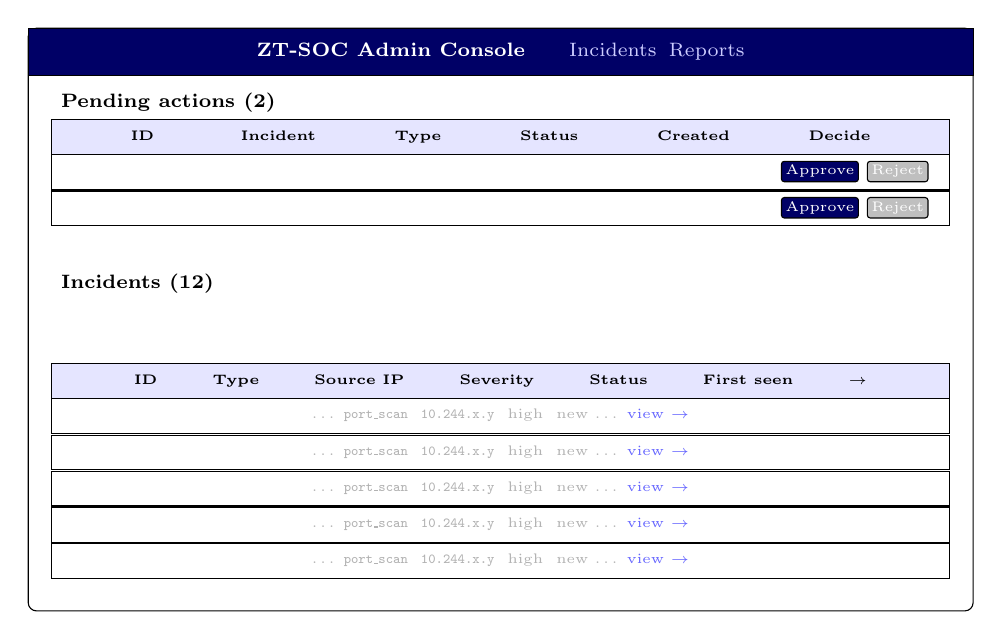
\begin{tikzpicture}[font=\scriptsize,
    win/.style ={draw, rounded corners=3pt},
    hbar/.style={draw, fill=blue!40!black, text=white, minimum height=0.6cm, align=left},
    hrow/.style={draw, fill=blue!10, minimum width=11.4cm, minimum height=0.46cm},
    row/.style ={draw, fill=white, minimum width=11.4cm, minimum height=0.44cm},
    btn/.style ={draw, rounded corners=1pt, fill=blue!40!black, text=white, font=\tiny, inner sep=1.5pt},
  ]
  \node[win, minimum width=12cm, minimum height=7.4cm] (w) {};
  \node[hbar, anchor=north west, minimum width=12cm] at (w.north west)
    {\textbf{ZT-SOC Admin Console}\quad\quad \textcolor{blue!20}{Incidents}\;\;\textcolor{blue!20}{Reports}};
  % Pending actions
  \node[anchor=north west, font=\scriptsize\bfseries] at ([xshift=0.3cm,yshift=-0.7cm]w.north west) {Pending actions (2)};
  \node[hrow, anchor=north] (ha) at (0,2.55) {};
  \node[font=\tiny\bfseries] at (0,2.32) {ID\hspace{1.1cm}Incident\hspace{1.0cm}Type\hspace{1.0cm}Status\hspace{1.0cm}Created\hspace{1.0cm}Decide};
  \foreach \i in {0,1}{
    \node[row, anchor=north] at (0,{2.1-\i*0.46}) {};
    \node[btn, anchor=east] at (4.55,{1.88-\i*0.46}) {Approve};
    \node[btn, fill=gray!50, anchor=west] at (4.65,{1.88-\i*0.46}) {Reject};
  }
  % Incidents
  \node[anchor=north west, font=\scriptsize\bfseries] at ([xshift=0.3cm,yshift=-3.0cm]w.north west) {Incidents (12)};
  \node[hrow, anchor=north] (hi) at (0,-0.55) {};
  \node[font=\tiny\bfseries] at (0,-0.78) {ID\hspace{0.7cm}Type\hspace{0.7cm}Source IP\hspace{0.7cm}Severity\hspace{0.7cm}Status\hspace{0.7cm}First seen\hspace{0.7cm}$\rightarrow$};
  \foreach \i in {0,...,4}{
    \node[row, anchor=north] at (0,{-1.0-\i*0.46}) {};
    \node[font=\tiny, gray!60] at (0,{-1.22-\i*0.46}) {\dots\ \texttt{port\_scan}\ \ \texttt{10.244.x.y}\ \ high\ \ new\ \dots\ \textcolor{blue!60}{view $\rightarrow$}};
  }
\end{tikzpicture}
}
  \caption{Wireframe màn hình Incidents (bảng hành động chờ duyệt $+$ bảng sự cố).}
  \label{fig:wf-incidents}
\end{figure}

Màn hình \textit{chi tiết sự cố} (Hình~\ref{fig:wf-detail}) là trung tâm thao tác: bảng
siêu dữ liệu (địa chỉ nguồn, mức độ, trạng thái, các nút quan sát được, cờ liên-nút, số
lần lặp, thời điểm đầu/cuối), bảng \emph{Actions} với nút duyệt, biểu mẫu \emph{Layer-2
follow-up} để lên lịch thao tác pod (\texttt{delete\_pod}/\texttt{shutdown\_pod} kèm
namespace, tên pod, lý do), và \emph{nhật ký kiểm toán} nhúng ngay trong trang.

\begin{figure}[H]
  \centering
  \resizebox{0.9\linewidth}{!}{% Wireframe (mockup) khop voi web-console THAT: trang chi tiet su co. Chuong 3.
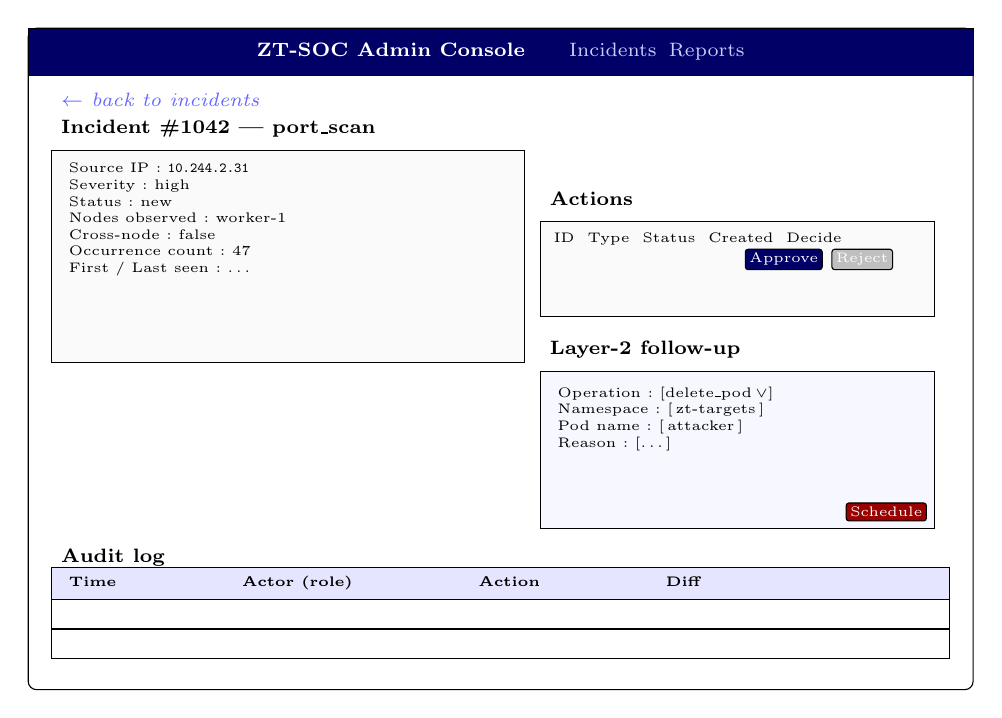
\begin{tikzpicture}[font=\scriptsize,
    win/.style ={draw, rounded corners=3pt},
    hbar/.style={draw, fill=blue!40!black, text=white, minimum height=0.6cm, align=left},
    panel/.style={draw, fill=gray!4},
    fld/.style ={draw, fill=white, minimum height=0.4cm},
    btn/.style ={draw, rounded corners=1pt, fill=blue!40!black, text=white, font=\tiny, inner sep=1.5pt},
  ]
  \node[win, minimum width=12cm, minimum height=8.4cm] (w) {};
  \node[hbar, anchor=north west, minimum width=12cm] at (w.north west)
    {\textbf{ZT-SOC Admin Console}\quad\quad \textcolor{blue!20}{Incidents}\;\;\textcolor{blue!20}{Reports}};
  \node[anchor=north west, font=\scriptsize\itshape, text=blue!60] at ([xshift=0.3cm,yshift=-0.7cm]w.north west) {$\leftarrow$ back to incidents};
  \node[anchor=north west, font=\scriptsize\bfseries] at ([xshift=0.3cm,yshift=-1.05cm]w.north west) {Incident \#1042 --- port\_scan};

  % Metadata table (2 cot)
  \node[panel, anchor=north west, minimum width=6.0cm, minimum height=2.7cm] (meta) at ([xshift=0.3cm,yshift=-1.55cm]w.north west) {};
  \node[anchor=north west, font=\tiny, align=left] at ([xshift=0.1cm,yshift=-0.05cm]meta.north west)
    {Source IP\ :\ \texttt{10.244.2.31}\\ Severity\ :\ high\\ Status\ :\ new\\ Nodes observed\ :\ worker-1\\ Cross-node\ :\ false\\ Occurrence count\ :\ 47\\ First / Last seen\ :\ \dots};

  % Actions table (ben phai metadata)
  \node[anchor=north west, font=\scriptsize\bfseries] at (0.5,2.25) {Actions};
  \node[panel, anchor=north west, minimum width=5.0cm, minimum height=1.2cm] (act) at (0.5,1.75) {};
  \node[font=\tiny, anchor=north west] at ([xshift=0.05cm,yshift=-0.03cm]act.north west) {ID \ Type \ Status \ Created \ Decide};
  \node[btn, anchor=north west] at ([xshift=2.6cm,yshift=-0.35cm]act.north west) {Approve};
  \node[btn, fill=gray!50, anchor=north west] at ([xshift=3.7cm,yshift=-0.35cm]act.north west) {Reject};

  % Layer-2 follow-up form
  \node[anchor=north west, font=\scriptsize\bfseries] at (0.5,0.35) {Layer-2 follow-up};
  \node[panel, fill=blue!3, anchor=north west, minimum width=5.0cm, minimum height=2.0cm] (fu) at (0.5,-0.15) {};
  \node[anchor=north west, font=\tiny, align=left] at ([xshift=0.1cm,yshift=-0.08cm]fu.north west)
    {Operation\ :\ [delete\_pod\,$\vee$]\\ Namespace\ :\ [\,zt-targets\,]\\ Pod name\ :\ [\,attacker\,]\\ Reason\ :\ [\dots]};
  \node[btn, fill=red!60!black, anchor=south east] at ([xshift=-0.1cm,yshift=0.1cm]fu.south east) {Schedule};

  % Audit log (duoi cung, ngang)
  \node[anchor=north west, font=\scriptsize\bfseries] at ([xshift=0.3cm,yshift=-6.5cm]w.north west) {Audit log};
  \node[draw, fill=blue!10, anchor=north west, minimum width=11.4cm, minimum height=0.4cm] (ah) at ([xshift=0.3cm,yshift=-6.85cm]w.north west) {};
  \node[font=\tiny\bfseries, anchor=west] at ([xshift=0.1cm]ah.west) {Time\hspace{1.6cm}Actor (role)\hspace{1.6cm}Action\hspace{1.6cm}Diff};
  \foreach \i in {0,1}{ \node[draw, fill=white, anchor=north west, minimum width=11.4cm, minimum height=0.38cm] at ([xshift=0.3cm,yshift={-7.25cm-\i*0.38cm}]w.north west) {}; }
\end{tikzpicture}
}
  \caption{Wireframe màn hình chi tiết sự cố.}
  \label{fig:wf-detail}
\end{figure}

Màn hình \textit{Reports} (Hình~\ref{fig:wf-reports}) tổng hợp báo cáo theo tuần: số sự cố,
trung vị thời gian phản hồi (MTTR), số sự kiện kiểm toán; phân tích theo mức độ, nguồn tấn
công nhiều nhất và loại hành động; cuối trang là biểu mẫu xuất nhật ký kiểm toán phục vụ
tuân thủ (định dạng CSV/JSON).

\begin{figure}[H]
  \centering
  \resizebox{0.86\linewidth}{!}{% Wireframe (mockup) khop voi web-console THAT: trang Reports (/reports). Chuong 3.
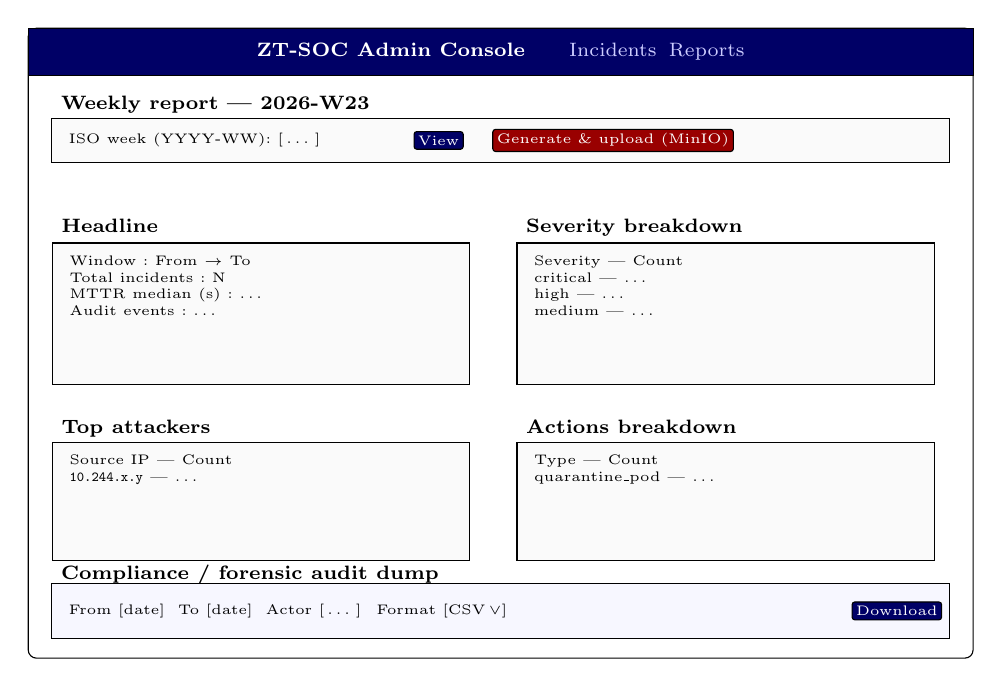
\begin{tikzpicture}[font=\scriptsize,
    win/.style ={draw, rounded corners=3pt},
    hbar/.style={draw, fill=blue!40!black, text=white, minimum height=0.6cm, align=left},
    panel/.style={draw, fill=gray!4},
    btn/.style ={draw, rounded corners=1pt, fill=blue!40!black, text=white, font=\tiny, inner sep=1.5pt},
  ]
  \node[win, minimum width=12cm, minimum height=8.0cm] (w) {};
  \node[hbar, anchor=north west, minimum width=12cm] at (w.north west)
    {\textbf{ZT-SOC Admin Console}\quad\quad \textcolor{blue!20}{Incidents}\;\;\textcolor{blue!20}{Reports}};
  \node[anchor=north west, font=\scriptsize\bfseries] at ([xshift=0.3cm,yshift=-0.75cm]w.north west) {Weekly report --- 2026-W23};
  % week selector + generate
  \node[panel, anchor=north west, minimum width=11.4cm, minimum height=0.55cm] (sel) at ([xshift=0.3cm,yshift=-1.15cm]w.north west) {};
  \node[anchor=west, font=\tiny] at ([xshift=0.1cm]sel.west) {ISO week (YYYY-WW): [\,\dots\,]\;\; };
  \node[btn, anchor=west] at ([xshift=4.6cm]sel.west) {View};
  \node[btn, fill=red!60!black, anchor=west] at ([xshift=5.6cm]sel.west) {Generate \& upload (MinIO)};

  % Headline
  \node[anchor=north west, font=\scriptsize\bfseries] at (-5.7,1.7) {Headline};
  \node[panel, anchor=north west, minimum width=5.3cm, minimum height=1.8cm] (hl) at (-5.7,1.28) {};
  \node[anchor=north west, font=\tiny, align=left] at ([xshift=0.1cm,yshift=-0.05cm]hl.north west)
    {Window\ :\ From $\rightarrow$ To\\ Total incidents\ :\ N\\ MTTR median (s)\ :\ \dots\\ Audit events\ :\ \dots};
  % Severity breakdown
  \node[anchor=north west, font=\scriptsize\bfseries] at (0.2,1.7) {Severity breakdown};
  \node[panel, anchor=north west, minimum width=5.3cm, minimum height=1.8cm] (sb) at (0.2,1.28) {};
  \node[anchor=north west, font=\tiny, align=left] at ([xshift=0.1cm,yshift=-0.05cm]sb.north west)
    {Severity\ |\ Count\\ critical\ |\ \dots\\ high\ |\ \dots\\ medium\ |\ \dots};
  % Top attackers
  \node[anchor=north west, font=\scriptsize\bfseries] at (-5.7,-0.85) {Top attackers};
  \node[panel, anchor=north west, minimum width=5.3cm, minimum height=1.5cm] (ta) at (-5.7,-1.25) {};
  \node[anchor=north west, font=\tiny, align=left] at ([xshift=0.1cm,yshift=-0.05cm]ta.north west)
    {Source IP\ |\ Count\\ \texttt{10.244.x.y}\ |\ \dots};
  % Actions breakdown
  \node[anchor=north west, font=\scriptsize\bfseries] at (0.2,-0.85) {Actions breakdown};
  \node[panel, anchor=north west, minimum width=5.3cm, minimum height=1.5cm] (ab) at (0.2,-1.25) {};
  \node[anchor=north west, font=\tiny, align=left] at ([xshift=0.1cm,yshift=-0.05cm]ab.north west)
    {Type\ |\ Count\\ quarantine\_pod\ |\ \dots};
  % Audit export form
  \node[anchor=north west, font=\scriptsize\bfseries] at ([xshift=0.3cm,yshift=-6.7cm]w.north west) {Compliance / forensic audit dump};
  \node[panel, fill=blue!3, anchor=north west, minimum width=11.4cm, minimum height=0.7cm] (ax) at ([xshift=0.3cm,yshift=-7.05cm]w.north west) {};
  \node[anchor=west, font=\tiny] at ([xshift=0.1cm]ax.west) {From [date] \ To [date] \ Actor [\,\dots\,] \ Format [CSV\,$\vee$]};
  \node[btn, anchor=east] at ([xshift=-0.1cm]ax.east) {Download};
\end{tikzpicture}
}
  \caption{Wireframe màn hình Reports (báo cáo tuần $+$ xuất nhật ký kiểm toán).}
  \label{fig:wf-reports}
\end{figure}

\section{Kết luận chương}

Chương này đã chuyển các yêu cầu và bài toán nêu ở Chương~\ref{ch:overview} thành một
thiết kế hệ thống cụ thể. Bắt đầu từ phân tích yêu cầu và mô hình mối đe dọa, chương đã
trình bày sơ đồ use-case cùng sơ đồ phân rã chức năng, rồi đặc tả kiến trúc phần mềm qua
sơ đồ mức container và các sơ đồ luồng dữ liệu, làm rõ vai trò của từng dịch vụ và đường
đi của dữ liệu trong hệ thống. Phần thiết kế cơ sở dữ liệu xác định các thực thể và quan
hệ phục vụ lưu vết sự cố, cảnh báo, hành động và nhật ký kiểm toán. Cuối cùng, chương đặc
tả quy trình phản hồi có người duyệt và thiết kế giao diện vận hành ở mức bố cục thành
phần. Toàn bộ thiết kế này là bản vẽ trực tiếp cho phần cài đặt và triển khai ở
Chương~\ref{ch:impl}.
